\documentclass{article}
\usepackage[utf8]{inputenc}

\usepackage{amsmath, amsthm, amssymb, amsfonts}

\usepackage{graphicx}

\theoremstyle{definition}
\newtheorem{exmp}{Example}[section]
\newtheorem{defn}{Definition}[section]

\newtheorem{theorem}{Theorem}[section]
\newtheorem{corollary}{Corollary}[theorem]
\newtheorem{lemma}[theorem]{Lemma}

\title{Notes for 36-733: Probability models and Stochatic Processes}
\author{Philipp Burckhardt}
\date{March 2015}

\begin{document}

\maketitle

\section{Introduction}

In Statistics, we often consider the case where data are iid (independent and identically distributed) observations from some underlying distribution $F_0$, i.e. $X_1, \ldots, X_n \sim F_0$. In regression analysis, we usually treat data as independent but coming from a different distribution:
$Y_i \mid X_i \sim N \left( \mu(X_i), \sigma^2 \right)$.
Our goal is to make inferences about the probabilities of some event involving $\vec{Y} = \left( Y_1, \ldots, Y_n \right)$:

$$
\Pr \left( \text{ some event involving } \vec{Y} \right) = \int_D f(\vec{y}) d\vec{y},
$$

when $Y \in D$. As one can see, we need access to the joint distribution to make inference on $\vec{Y}$. 
In case that the data are independent, we have

$$
f_{\vec{Y}} \left( \vec{y} \right) = \prod_{i=1}^n f_{Y_i} \left(y_i \right)
$$

In this course, we treat dependent data. We therefore have to postulate a $n$-dimensional model, which in turn means that we need much larger samples for drawing inference because of the added complexity and the dependence in the data.
Specifically, we will treat the following cases:
\begin{enumerate}
\item Data as time processes
\item Data have Markov property
\end{enumerate}

Recall the definition of conditional probability:

$$
P (A \mid B) P(B) = P(A, B)
$$

$$
f_{\vec{Y}} \left( \vec{y} \right) = f_{Y_n} ( y_n \mid \vec{Y}_{n-1} ) f_{\vec{Y}_{n-1}} ( \vec{y}_{n-1} ) = \left[ \prod_{i=2}^n f_{Y_i} (y_i \mid Y_1, \ldots, Y_{i-1} ) \right] f_{Y_1} (y_1)
$$

\begin{exmp}
$Y_t \mid Y_{t-1} \sim N \left( Y_{t-1}, \sigma^2 \right)$
\end{exmp}

\section{Discrete time, discrete state space Markov chain}

We assume that the state space $S$ is discrete or countable. The state space denotes the possible values the random variables int he chain can take: $X_n \in S$.

\begin{defn}{Markov Property:} 
$$
\forall n > 0, \forall m > 0 \quad P\left( X_{m+n} = s \mid X_0 = x_0 , \ldots, X_m = x_m \right) = P \left( X_{m+n} = s \mid X_m = x_m \right) 
$$
\end{defn}

To introduce some simplifying notation, let us define

$$
p_{ij} = P(X_{n+1} = j \mid X_n = i) \qquad \forall (i,j) \in S^2 \quad \forall n \in \mathbb{N}.
$$

Notice that the $p_{ij}$ are assumed to stay constant over time. We have 

$$
p( \vec X ) = p(X_0) \prod_{i=1}^n p(X_i \mid X_{i-1})
$$

\begin{exmp}
$S = \{ \text{wet, dry} \}$. Then 
$$
P \left(X_{\text{Jan 2}} = \text{wet} \mid X_{Jan 1} = \text{wet} \right) \ne P \left(X_{\text{Jul 2}} = \text{wet} \mid X_{\text{Jul 1}} = \text{wet} \right),
$$
so this is not a \emph{stationary} process.
\end{exmp}

\begin{defn}
Transition Matrix:
$$
P = \left[ p_{ij} \right], \qquad (i,j) \in S^2
$$
\end{defn}

In the following examples, answer the following questions 

\begin{enumerate}
\item Is it a Markov chain?
\item What is $P$?
\end{enumerate}

\begin{exmp} Simple Random Walk: Drunken Man on a Line. We assume that $X_t = X_{t-1} + 1$ with prob $p$ and $X_t = X_{t-1} - 1$ with prob $1-p$.
\end{exmp}

\begin{exmp} Random Walk with Self-Absorbing barriers: Gambler's Ruin. When $X_t = N$ or $X_t = 0$, the chain stays in the respective state forever. 
\end{exmp}

\begin{exmp} Inventory Problem:
$X_n = \text{\# Paper Towel boxes left at day n}$.
If $X_n = 0$, we order $2$ boxes which magically arrive over night. If $X_n > 0$, we do not place an order. Let $\xi = \text{ \# boxes used per day}$. We have $P(\xi = 0) = 0.5, P(\xi = 1) =0.4$ and $P(\xi = 2) = 0.1$.
\end{exmp}

\subsection{Questions of Interest}
Two main categories of quantities of interest are the probabilities of events and the expected number of steps until a certain event happens. 

Consider the following example in Figure \ref{fig:interest_plot01}:

\begin{figure}[h!]
\centering
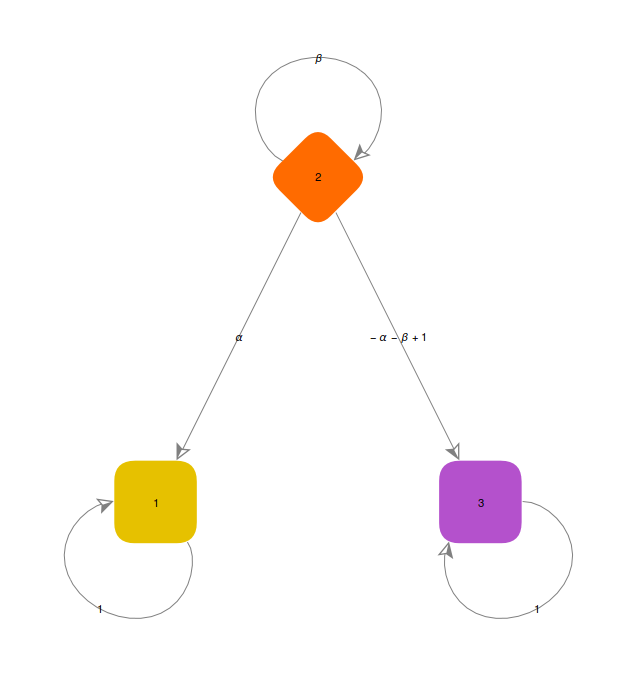
\includegraphics[width=0.75\textwidth]{images/interestPlot01}
\caption{Example of a Markov Chain}
\label{fig:interest_plot01}
\end{figure}

The corresponding transition matrix is 

$$
P = \begin{pmatrix}
1 & 0 & 0 \\
\alpha & \beta & \gamma  \\
0 & 0 & 1 \\
\end{pmatrix},
$$

where $\gamma = 1 - \alpha - \beta$. We are interested in the event of absorption in the first state given that the chain starts in state $2$. Define $ W= \cup_{i=0}^\infty \{X_i = 1\}$. Our quantity of interest thus is $P(W \mid X_0 = 2)$. 

We have

$$
P(W \mid X_0 = 2) = \sum_{i=1}^3 P(W \mid X_0 = 2, X_1 = i) P(X_1 = i \mid X_0 = 2).
$$

Observe that 

\begin{align*}
 P(W \mid X_0 = 2, X_1 = 1) &= 1 \\
 P(W \mid X_0 = 2, X_1 = 3) &= 0 \\
  P(W \mid X_0 = 2, X_1 = 2) &=  P(W \mid X_0 = 2)
\end{align*}

To prove the last equality rigorously, let us use the definition of $W$:

\begin{align*}
  P(W \mid X_0 = 2, X_1 = 2) &= 
  P \left( \cup_{i=1}^\infty \{X_i = 1\}  \mid X_0 = 2, X_1 = 2 \right) \\ 
  &=  P \left( \cup_{i=2}^\infty \{X_i = 1\} \mid X_0 = 2, X_1 = 2 \right) \\
  &= P \left( \cup_{i=2}^\infty \{X_i = 1\} \mid X_1 = 2 \right ) \; \text{[because of Markov property]} \\
    &= P \left( \cup_{i=1}^\infty \{X_i = 1\} \mid X_0 = 2 \right) \; \text{ [because of Time-Homogeneity] }
\end{align*}

Next, we consider $E \left[ \text{\# steps till absorbed} \mid X_0 = 2 \right]$. We have

$$
E \left[ \text{\# steps till absorbed} \mid X_0 = 2 \right] = \sum_{i=1}^3 E \left[ \text{\# steps till absorbed} \mid X_0 = 2, X_1 = i \right] P(X_1 = i \mid X_0 = 2).
$$

Plugging in, we get
$$
E = \alpha + \beta (1 + E) + \gamma
$$

which solving for $E$ gives us the result $E= \frac{1}{1-\beta} = \frac{1}{\alpha + \gamma}$.

\subsubsection*{First-Step Analysis} 
Define $T = \text{\# steps till absorbed}$. We have just shown that 

$$
E\left[T \mid X_0 = 2 \right] =  \frac{1}{1-\beta}.
$$

By definition, we have

$$
E\left[T \mid X_0 = 2 \right] = \sum_{t=1}^\infty t \, P(T=t\mid X_0 = 2).
$$

Since $T \sim \text{Geometric}(1-\beta)$, we know that 
$$
P(T=t\mid X_0 = 2) = (1 - \beta)\,\beta^{t-1},
$$

so we could have also obtained the result via this route:


\begin{align*}
E\left[T \mid X_0 = 2 \right] 
&= \sum_{t=1}^\infty t \,  \beta^{t-1}\,(1-\beta) \\
&= \frac{1}{1-\beta} \quad \text{ [mean of Geometric r.v with parameter $1-\beta$]}
\end{align*}

$$
E \left[ T \mid X_0 = 2, X_1 = 2 \right] \overset{?}{=} 1 + E \left[ T \mid X_0 = 2 \right]
$$

\begin{proof}

\begin{align*}
E \left[ T \mid X_0 = 2, X_1 = 2 \right] 
&= \sum_{t=1}^\infty t P \left( X_t \ne 2, X_i = 2, i=1,\ldots,t-1 \mid X_0 = 2, X_1 = 2 \right) \\
&= \sum_{t=1}^\infty t P \left( X_{t-1} \ne 2, X_1 = 2, \ldots, X_{t-2} \mid X_0 = 2 \right) \\
&= \sum_{t=1}^\infty (t-1) P \left( X_t \ne 2,  X_1 = 2, \ldots, X_{t-1} = \mid X_0 = 2, X_1 = 2 \right) \\
&\qquad \qquad + \sum_{t=1}^\infty P \left( X_t \ne 2, X_1 = 2, \ldots, X_{t-1} = 2 \mid X_0 = 2, X_1 = 2 \right) \\ 
&= E\left[T \mid X_0 = 2 \right] +1
\end{align*}

\end{proof}

Since it is possible that the chain is absorbed into state $3$, we have

$$
E \left[ \text{\# steps till absorbed at state 1} \mid X_0 = 2 \right] = \infty.
$$

Probably, we would rather be interested in this expectation conditional on the fact that the chain is absorbed at state $1$. Let $W$ be a random variable denoting that the chain is absorbed into state $1$. We would thus like to calculate 
\begin{align*}
&E \left[ \text{\# steps till absorbed at state 1} \mid X_0 = 2, W \right] \\
&= E \left[ T \mid X_0 = 2, X_1 = 2, W \right] P(X_1 = 2 \mid X_0 = 2, W) \\
&\qquad \qquad + E \left[ T \mid X_0 = 2, X_1 = 1, W \right] P(X_1 = 1 \mid X_0 = 2, W).
\end{align*}

To shorten the notation, define $E^\star[\cdot] = E[\cdot \mid W]$. We then have

\begin{align*}
&E^\star \left[ T \mid X_0 =2 \right] = (1 + E^\star \left[ T \mid X_0 = 2 \right]) P^\star (X_1 =2 \mid X_0 = 2) + P^\star (X_1 = 1 \mid X_0 =2) \\
&\iff E^\star \left[ T \mid X_0 =2 \right] = (1 + E^\star \left[ T \mid X_0 = 2 \right]) \frac{\beta}{\alpha+\beta} + \frac{\alpha}{\alpha+\beta}
\end{align*}

We conclude that 

$$
E^\star \left[ T \mid X_0 =2 \right] = \frac{\alpha+\beta}{\alpha} = \frac{1}{\alpha/(\alpha+\beta)} = \frac{1/p(2\to1)}{p(2\to1 \text{ or } 2 \to 2)}
$$

\begin{defn}[Mean Recurrence Time] The mean recurrence time for state $i \in S$ is defined as 
$$
m_i = E \left[ \text{\# steps till chain first returns to i} \mid X_0 = i \right]
$$
\end{defn}

In our example we have $m_1 = 1, m_2 = \infty, m_3 = 1$.

\subsection{Random Walks}

$$
X_{t + \tau} = X_t + \varepsilon_{t + \tau}, \quad \tau \in \mathbb{R}^+
$$

Example of a random walk: Stock prices on the stock exchange. 

$\tau = 1,2,\ldots$.

$$
X_{n+1} = X_n + \varepsilon_{n+1}
$$

In a simple random walk, $\varepsilon$ are iid. In this case, the process is a Markov chain. 

\begin{exmp}[Gambler's Ruin]
Let $p \in (0,1)$. The MC is defined as follows:
$X_{n+1} = X_n + 1$ with prob $p$ and $X_{n+1} = X_n -1$ with prob $q=1-p$. The gambler has an initial wealth of $X_0 = \$k$. When $X_i = 0$, he is ruined, whereas he has become rich (and stops playing) when $X_i = N$. 
\end{exmp}

We might be interested in the event that the gambler is ruined. Let us define $p_k = \Pr \left( \text{ruin} \mid X_0 = k \right)$, where $k \in \{0, \ldots, N\}$. 
Notice that we have the boundary conditions $p=0 = 1$ and $p_N = 0$. In addition, we have the following recurrence relation:

$$
p_k = p \, p_{k+1} + q \, p_{k-1} \iff 0 = p \, p_{k+1} + q \, p_{k-1} - p_k
$$

This is a second order linear difference equation. It is homogeneous because the left-hand side is equal to zero. 

We can solve it as follows: 
\begin{align*}
&p_i = p \, p_{i+1} + q \, p_{i-1} \\
&\iff p p_i + q p_i = p p_{i+1} + q p_{i-1} \\
&\iff p_{i+1} - p_i = \tfrac{q}{p} \left( p_i - p_{i-1} \right) 
\end{align*}

We get
\begin{align*}
&p_2 - p_1 = \tfrac{q}{p} \left( p_1 - p_{0} \right) =  \tfrac{q}{p} p_1 \\
&p_3 - p_2 =  \tfrac{q}{p} \left(p_2 - p_1 \right) = \left( \tfrac{q}{p} \right)^2 p_1 \\
&p_{i+1}-p_i = \left( \tfrac{q}{p} \right)^i p_1 \text{ for } 0 < i < N
\end{align*}

It follows that 

\begin{align*}
&p_{i+1} - p_1 = \sum_{k=1}^i \left( \tfrac{q}{p} \right)^k p_1 \\
&\iff p_{i+1} = p_1 + \sum_{k=1}^i \left( \tfrac{q}{p} \right)^k p_1 = \sum_{k=0}^i \left( \tfrac{q}{p} \right)^k p_1 = \begin{cases} p_1 (i+1) & \text{ if } q = p \\
p_1 \frac{1-\left( \tfrac{q}{p} \right)^{i+1}}{1-\tfrac{q}{p}} & \text{ if } q \ne p\end{cases}
\end{align*}

With the boundary conditions:

$$
p_N = 1 = \begin{cases} p_1 N & \text{ if } q = p \\
p_1 \frac{1-\left( \tfrac{q}{p} \right)^{N}}{1-\tfrac{q}{p}} & \text{ if } q \ne p\end{cases} \implies p_1 = \begin{cases} \frac{1}{N} & \text{ if } q = p \\
 \frac{1-\left( \tfrac{q}{p} \right)^{1}}{1-\left( \tfrac{q}{p} \right)^N} & \text{ if } q \ne p\end{cases}
$$

More generally, we get 
$$
 p_i = \begin{cases} \frac{i}{N} & \text{ if } q = p \\
 \frac{1-\left( \tfrac{q}{p} \right)^{i}}{1-\left( \tfrac{q}{p} \right)^N} & \text{ if } q \ne p\end{cases}
$$

Recall to always keep in mind what you are conditioning on. It is easy to make mistakes in that regard. 

Consider the following difference equation and boundary conditions:

\begin{align*}
&p_k = p \, p_{k+1}  + q \, p_{k-1} \qquad k \in \{0, 1, \ldots, N\}\\
&p_0 = 1 \\
&p_N = 1\\
\end{align*}

We rewrite it: 

$$
0 = -p_k + p \, p_{k+1} + q \, p_{k-1} \implies p(x) = -x + px^2 + \frac{q}{p}
$$

$p(x)$ is the characteristic polynomial, for which we first calculate its roots:

$$
x_{1,2} = \frac{1}{2p} \pm \sqrt{\frac{1}{p^2} - \frac{q}{p}} \implies x_1 = 1 \text{ and } x_2 = \frac{q}{p}
$$

\subsection{Appendix A: Linear Difference Equations with Constant Coefficients}

\subsubsection{Homogeneous Case}

$$
p_n = c_1 p_{n-1} + c_2 p_{n-2} + \ldots + c_d p_{n-d}
$$

Current term depends on $d$ previous terms. This is an ordered linear difference equation with constant coefficients. Since there is no constant term, we are dealing with the \emph{homogeneous case}. 

We rewrite the equation as 

$$
0 = p_n - c_1 p_{n-1} - c_2 p_{n-2} + \ldots - c_d p_{n-d}
$$

Setting $n = d$, we get

$$
0 = p_d - c_1 p_{d-1} - c_2 p_{d-2} - \ldots - c_d p_{0}
$$

By replacing $p_i$ with $x^i$, we obtain the characteristic polynomial:

$$
p(x) = x^d - c_1 x^{d-1} - c_2 x^{d-2} - \ldots - c_d = 0
$$

We find the roots of the characteristic polynomial, i.e. the values which make it zero. There are at most $d$ roots- 
Then solution to difference equation is 

\begin{align*}
p_n =  x_1^n \times \left[ A_11 + A_12 n + A_13 n^2 + \ldots A_{1n} n \right]
\end{align*}

We need $d$ values

\subsubsection{Inhomogeneous Case}

$$
p_n = c_1 p_{n-1} + c_2 p_{n-2} + \ldots + c_d p_{n-d} + K 
$$

This is the \emph{imhomogeneous case} because of the constant $K$ which does not depend on $n$.
The solution is

$$
p_n = \text{solution to homogeneous eq.} + \text{particular solution}
$$

To calculate the particular solution, one has to find some $p_n$ which satisfies the equation. There is no foolproof way to do this and solutions might not be unique. The coefficients are then determined using the boundary conditions. 

If particular solution cannot be found, one can reduce the inhomogeneous equation to homogeneous one by differentiation:

\begin{exmp}

\begin{align*}
p D_{k+1} + q D_{k-1} + 1 - D_k = 0 \\
p D_{k+2} + q D_k + 1 - D_{k+1} = 0
\end{align*}

The difference yields a homogeneous equation of order three:

$$
\Delta = p D_{k+2} + q D_k - D_{k+1} - p D_{k+1} - q D_{k-1} + D_k
$$
\end{exmp}

We then have to find the roots of the third order polynomial, which is not an easy task as there is no systematic method. However, in case of linear equations, it is usually possible to find solutions. 

\section{Long-Run Behaviour of Markov Chains}
We consider the situation when $n$ large, $n \to \infty$.

If 
$P \left( X_n = j \mid X_0 = i \right) = P \left( X_n = j \right) = P(X = j)$ independent of $i$ for $n > n_0$ large, then $\vec{\pi}$ with elements $\pi_j = P(X = j)$ denotes the limiting distribution of the MC.

If a limiting distribution exists, we have for large $n$

$$
P(n) = \left[ p_{ij}(n) = P(X_n=j \mid X_0 = i)  \right]_{i,j} \to \begin{pmatrix} \vec{\pi} \\ \vdots \\ \vec{\pi} \\ \end{pmatrix}
$$

We also have $P(n) = P^n$ following from the Chapman-Kolmogorov Equations. This gives us two options to find the limiting distributions $\pi$:

\begin{enumerate}
\item Find $\pi$ using $P^n$ for large $n$.
\item Find a stationary distribution and if limiting distribution exists, stationary distribution is equal to it.
\end{enumerate}

Let us denote $\mu_i^0 = P(X_0 = i)$ and $\vec{\mu}^0_i = \left( P(X_0 = 0), \ldots \right)$

A stationary distribution $\delta$ is such that  
$$
\vec{\mu}^0 = \vec{\delta} \implies \forall n \in \mathbb{N}: \vec{\mu}^n = \vec{\delta}
$$

Observe that 

$$
p(X_1 = j) = \sum_{i \in S} P(X_1 = j \mid X_0 = i ) P(X_0 = i) \implies \vec{\mu}^1 = \vec{\mu}^0 P.
$$

The stationary distribution satisfies $ \vec \delta = \vec \delta P$.

\begin{theorem}[Chapman-Kolmogorov-Equation]
$$
\forall (m, n, r) \in \mathbb{N}^3 \qquad P(m + r) = P(m) P(r).
$$
So we have for example $P(2) = P P = P^2$ and $P(n) = P^n$. 
\begin{proof}
By the law of total probability, we have

\begin{align*}
&P \left( X_{m + n + r} = j \mid X_m = i \right) \\
&\qquad = \sum_{k \in S} P \left( X_{m + n} = k \mid X_n = i \right) P \left( X_{m + n + r} = j \mid X_{n+m} = k \right)
\end{align*}

Hence for all $i,j$ we have

$$
P_{ij}(m+r) = \sum_{k \in S} P_{ik}(m) P_{kj}(r) \implies P(m+r) = P(m) P(r).
$$

\end{proof}
\end{theorem}

\subsubsection*{Examples}

\begin{figure}[h!]
\centering
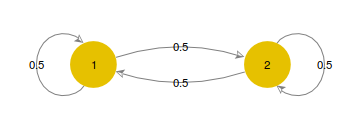
\includegraphics[width=0.8\textwidth]{images/exmc1}
\label{fig:exmc1}
\caption{ The limiting and stationary distribution of this MC is given by $\vec \pi = [0.5, 0.5]$.}
\end{figure}

\begin{figure}[h!]
\centering
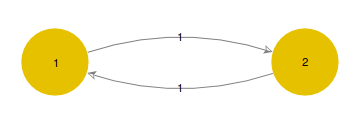
\includegraphics[width=0.5\textwidth]{images/exmc2}
\label{fig:exmc2}
\caption{ The stationary distribution of this MC is given by $\vec \pi = [0.5, 0.5]$. However, the MC does not have a limiting distribution because of its periodic nature.}
\end{figure}

\begin{figure}[h!]
\centering
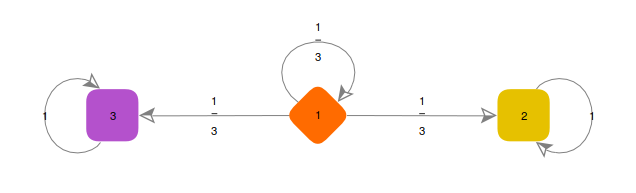
\includegraphics[width=0.8\textwidth]{images/exmc3}
\label{fig:exmc3}
\caption{Since there cannot be a limiting distribution whenever there is an absorbing state, we only try to find a stationary distribution: In this case, an infinite number of such distributions exist: $\delta_1 = (0,1,0)$ and $\delta_2 = (0,0,1)$ work, and also any convex combination of these two states: $\delta_3 = \alpha \delta_1 + (1-\alpha) \delta_2$ for $\alpha \in [0,1)$.}
\end{figure}


\subsection{Classification of States}

\begin{defn}[Persistent vs. Transient]
A state is called \emph{persistent} or \emph{recurrent} if $P( \text{ return to j } \mid X_0 = j) = 1$ (in whatever number of steps). Otherwise it is called \emph{transient}.
\end{defn}

\begin{defn}[Positive vs. Null]
A state is positive or non-null if its mean recurrence time is finite, i.e. 
$E\left[ \text{ \# steps to return} \right] < \infty$. If $E\left[ \text{ \# steps to return} \right]~=~\infty$, the state is said to be null.
\end{defn}

\begin{defn}[Periodic]
Positive non-null states can be further divided into whether they are periodic or non-periodic. 
The period of state $x \in S$ is given by
$$
d(x)= gcd \{n \in \mathbb{N}+: p_{xx}(n)>0 \}.
$$
\end{defn}

\begin{defn}[Ergodic]
A state $x \in S$ is ergodic iff it is
\begin{enumerate}
\item persistent
\item non-null
\item non-periodic.
\end{enumerate}
\end{defn}

\begin{exmp}[Simple Random Walk with Absorbing Barriers]
Consider the SRW with absorbing states at $0, N$, where $N > 1$. The states $0,N$ are persistent with mean recurrence times $m_0 = m_N = 1$, i.e. they are also non-null. Finally, they are aperiodic. In contrast, all other states are transient, null since $m_j = \infty$ and have period $2$.
\end{exmp}

\begin{exmp}[Simple Random Walk]
For the simple random walk with $S = \mathbb{Z}$, $p \in (0,1)$, the results depend on $p$. For $p \ne 1/2$, all states are transient. However, for $p=1/2$, the chain returns with probability $p=1$, hence states are persistent. However, they are again null and periodic, where the period is $2$.
\end{exmp}

\begin{theorem}
A persistent state $j$ is null if and only if $p_{jj}(n) \to 0$ as $n \to +\infty$.
\end{theorem}

\begin{align*}
E_{11} 
&= \frac{1}{2} E(T \mid X_0 = 1, X_1 = 1) + \frac{1}{2}  E(T \mid X_0 = 1, X_1 = 2) \\
&= \frac{1}{2} + \frac{1}{2} ( 1 + E_{21} ) 
\end{align*}

\begin{defn}[Irreducibility]
A chain is irreducible if $
\forall (i,j) \in S^2 \, \exists (m,n)$ such that 
$$
p_{ij}(m) > 0 \text{ and } p_{ji}(n) > 0.
$$
\end{defn}

\begin{theorem}
If $S$ is inite, there is at least one persistent state and all persistent states are positive.
\end{theorem}

\begin{theorem}
If $i \leftrightarrow j$, then 
\begin{enumerate}
\item $i$ and $j$ have the same period.
\item $i$ transient if and only if $j$ is transient 
\item $i$ persistent if and only if $j$ is persistent
\item $i$ null persistent if and only if $i$ is. 
\end{enumerate}
\end{theorem}

\begin{lemma}
If $S$ is finite and the MC is irreducible, then all states are persistent non-null and have the same period.
\end{lemma}

\begin{theorem}
An irreducible chain has a stationary distribution $\delta$ if and only if all states are positive persistent. Then $\delta$ is unique and satisfies
$$
\delta = \delta P \qquad \delta_i \ge 0 \qquad \sum \delta_i = 1.
$$
We do not have a similar statement for reducible Markov chains. 
\end{theorem}

\begin{theorem}
For an irreducible, aperiodic chain
$$
\forall (i,j) \qquad  p_{ij}(n) \to \frac{1}{m_j} \text{ as } n \to \infty,
$$
where $m_j = E \left[ \text{ \# steps to first return to j} \mid X_0 = j \right]$ is the \emph{mean recurrence time}.
\end{theorem}

\begin{theorem}
If the chain is irreducible and ergodic, then the limiting distribution exists, is unique and is given by
$$
p_{ij}(n) \to \frac{1}{m_j}.
$$
\end{theorem}

\subsection{Reducible Chains}

\begin{theorem}[Decomposition Theorem]
The state space $S$ can be decomposed $S = T \cup C_1 \cup C_2 \ldots$, where $T$ is a set of transient states and the $C_i$ are closed, irreducible persistent states.
\end{theorem}

\begin{exmp}[SRW]
$X_0 = k$, $X_i = X_{i-1} + 1$ with prob $p$ and $X_{i} = X_{i-1} -1$ with prob $q$.
We have
$$
p_k = P(\text{return to k} \mid X_0 = k)
$$

First-step Analysis:

$$
p_k = P(R \mid X_0 = k) = p p_{k+1} + q p_{k-1} = P(R \mid X_0 = k, X_1 = k+1) \, p + P(R \mid X_0 = k, X_1 = k-1) \, q
$$

$$
P(A \mid X_0 = 0) = P \left( \cup_{i=1}^\infty B_i \mid X_0 = 0 \right),
$$

where $B_i = \{ X_i = 0 \text{ and } X_j \ne 0, \forall \, 1 \le j < i\}$.

Since the events are disjoint, we have

$$
P \left( \cup_{i=1}^\infty B_i \mid X_0 = 0 \right) = \sum_{i=1}^\infty P(B_i \mid X_0 = 0)
$$

Let us define $f_{00}(i) =  P(B_i \mid X_0 = 0)$.

$$
p_{00}(i) = P(\text{ return to 0 in i steps} \mid X_0 = 0) = \begin{cases}
0 & \text{ if i odd} \\
{ i \choose i/2} p^{i/2} q^{i/2} & \text{ if i even} 
\end{cases}
$$

\begin{align*}
p_{00}(i) = p(X_i = 0 \mid X_0 = 0) 
&= \sum_{k=1}^i P(X=0 \mid B_k, X_0 = 0) P(B_k \mid X_0 = 0) \\
&=  \sum_{k=1}^i p_{00}(i-k) f_{00}(k)
\end{align*}

$$
\implies p_i = \sum_{k=1}^i p_{i-k} f_k
$$

Inhomogeneous recurrence equation of order $i$ for $f_k$.


\begin{defn}[Generating functions (GF)]
The GF of a sequence $a_0, a_1, a_2 \in \mathbb{R}$ is $G_a(s) = \sum_{i=0}^\infty a_i s^i$. $G'_a(s) = \sum_{i=1}^\infty i a_i s^{i-1}$.
\end{defn}

$$
a_i = f_{00}(i) = P(B_i \mid X_0 = 0)
$$

$$ 
F_{00}(s) = \sum_{i=0}^\infty f_{00}(i) s^i,
$$

with $f_{00}(0) = 0$. 

$$
p_{00}(s) = \sum_{i=0}^\infty p_{00}(i) s^i,
$$

Since we have
$p_{00}(i)  = \begin{cases}
0 & \text{ if i odd} \\
{ i \choose i/2} p^{i/2} q^{i/2} & \text{ if i even} 
\end{cases}$, we get

$$
p_{00}(s) = \sum_{i=0}^\infty { 2i \choose i} \left( p \, q \, s^2 \right)^i = (1-4pqs^2)^{-1/2}
$$

Observe:

$$
p_{00}(1) = \sum p_{00}(i) = (1-4pq)^{-1/2}
$$

Observe that if $p=q$, this quantity is infinity.

\begin{defn}[Convolution]
Continuous case:
$$
\int g(y-x) f(x) dx 
$$
Discrete case:
$$
\sum_{k=0}^i g_{i-k} f_k
$$
\end{defn}

\begin{theorem}
Let us consider two sequences $a_0, a_1, \ldots$ and $b_0, b_1, b2$ with generating functions $G_a(s)$ and $G_b(s)$ then 
$c_0,c_1,c_2$ where $c_k = \sum_{i=0}^k a_i b_{k-i}$, then 
$G_c(s) = G_a(s) \, G_b(s)$.

\begin{proof}
$$
G_a(s) G_b(s) = \left( \sum_{i=0}^\infty a_i s^i \right) \left( \sum_{j=0}^\infty b_j s^j \right) = \sum_{k=0}^\infty c_k s^k,
$$

where $c_k = \sum_{(i,j) \text{s.t.} i+j=k} a_i b_j = \sum_{i=0}^k a_i b_{k-i}$.
\end{proof}
\end{theorem}

We have proven that $p_{00}(i) = \sum_{k=1}^i p_{00}(i-k) f_{00}(i)$ for $i \ge 1$. When $p=0$, $p_{00}(0) = 1$ and $f_{00}(0) = 0$.

\end{exmp} 

\subsection{Reversible Chains}

Let $\{X_n\}$ be an irreducible, persistent, positive MC ($\implies !\exists \text{ stationary distribution } \pi$). 

$$
\forall n \, X_n \sim \pi.
$$

$N$ large, $Y_n = X_{N-n}$.

\begin{theorem}
$Y_n$ is a MC with transition probabilities 
$$
q_{ij} = p_{ji} \frac{\pi_j}{\pi_i}
$$
\begin{proof}

\begin{align*}
    \forall n \, P\left( Y_n = j \mid Y_{n-1} = i, Y_{n-2} = k, \ldots \right) 
    &= P \left( X_{N-n} = j \mid X_{N-(n-1)} = i, X_{N-(n-2)}=k \right) \\
    &= \frac{P \left( X_{N-n} = j, X_{N-(n-1)} = i, X_{N-(n-2)}=k \right) }{P \left( X_{N-(n-1)}=i, X_{N-(n-2)} = k\right)} \\
    &= \frac{P(X_{N-(n-1)} = i \mid X_{N-n} = j) P(X_{N-n} = j) }{P(X_{N-(n-1)})} \\
    &= p_{ji}  \frac{\pi_j}{\pi_i}
\end{align*}

\end{proof}
\end{theorem}

\begin{defn}
A MC is called reversible if 
$$
\forall (i,j) \, p_{ij} = q_{ij}
$$
\end{defn}

$$
\implies \pi_i p_{ij} = \pi_j p_{ji} \quad \pi \text{ is in detailed balance with} P
$$

\begin{theorem}
Let $P$ be transition matrix of irreducible chain. Suppose $\exists$ distribution $\pi$ s.t. $\forall (i,j) \in S^2 \, \pi_i p_{ij} = \pi_j p_{ji}$,
then $\pi$ is a stationary distribution of the Markov chain. 

\begin{proof}
We prove that $\pi = \pi P$. 
$$
\forall i \, \pi_i = \sum_j \pi_j p_{ji}
$$

\end{proof}
\end{theorem}

\section{Markov Chain Monte Carlo (MCMC)}
MCMC = art of building MC with specified limiting distributions.

Let $f_X(x)$ be a distribution, we want $E(X) = \int x f(x) \, dx$. 

\section{Continuous Time Processes}

\subsection{Properties of Poisson Process}

\subsubsection{Inter-arrival \& Wait Times}

$$
T_i = \sum_{j=1}^i X_j \qquad X_i = T_i - T_{i-1}
$$

\begin{theorem}
If the process is Poisson, then
\begin{enumerate}
\item $X_i \overset{iid}{\sim} \exp(\lambda)$
\item $\forall k, T_k \sim \Gamma(k, \lambda)$
\end{enumerate}
\begin{proof}
\begin{enumerate}
\item $F_X(x) = P(X_i \le x)$. Can do it in terms of $T$'s: $P(T_i - T_{i-1} \le x)$, but joint distribution very hard. So let's do it in terms of $N(t)$'s:
First: $X_1 = T_1 \implies f_X(t) = \lambda e^{-\lambda t}$. But we don't get far. 
\item $\forall t$, find $F_{T_k}(t) = P(T_k \le t) = P(N(t) \ge k) = \sum_{j=k}^\infty \tfrac{(\lambda t)^j e^{-\lambda t}}{j!}$.
Let's try: $f_{T_k} = F_{T_k}'(t)$. The derivative is 
$\frac{\lambda^k t^{k-1} e^{-\lambda t}}{(k-1)!}$, the pdf of a $\Gamma(k, \lambda)$ distribution. 
\end{enumerate}
\end{proof}
\end{theorem}





\end{document}
